\documentclass[border=8pt]{standalone}
\usepackage{tikz}
\usetikzlibrary{arrows.meta,positioning,fit,backgrounds,calc}
\begin{document}
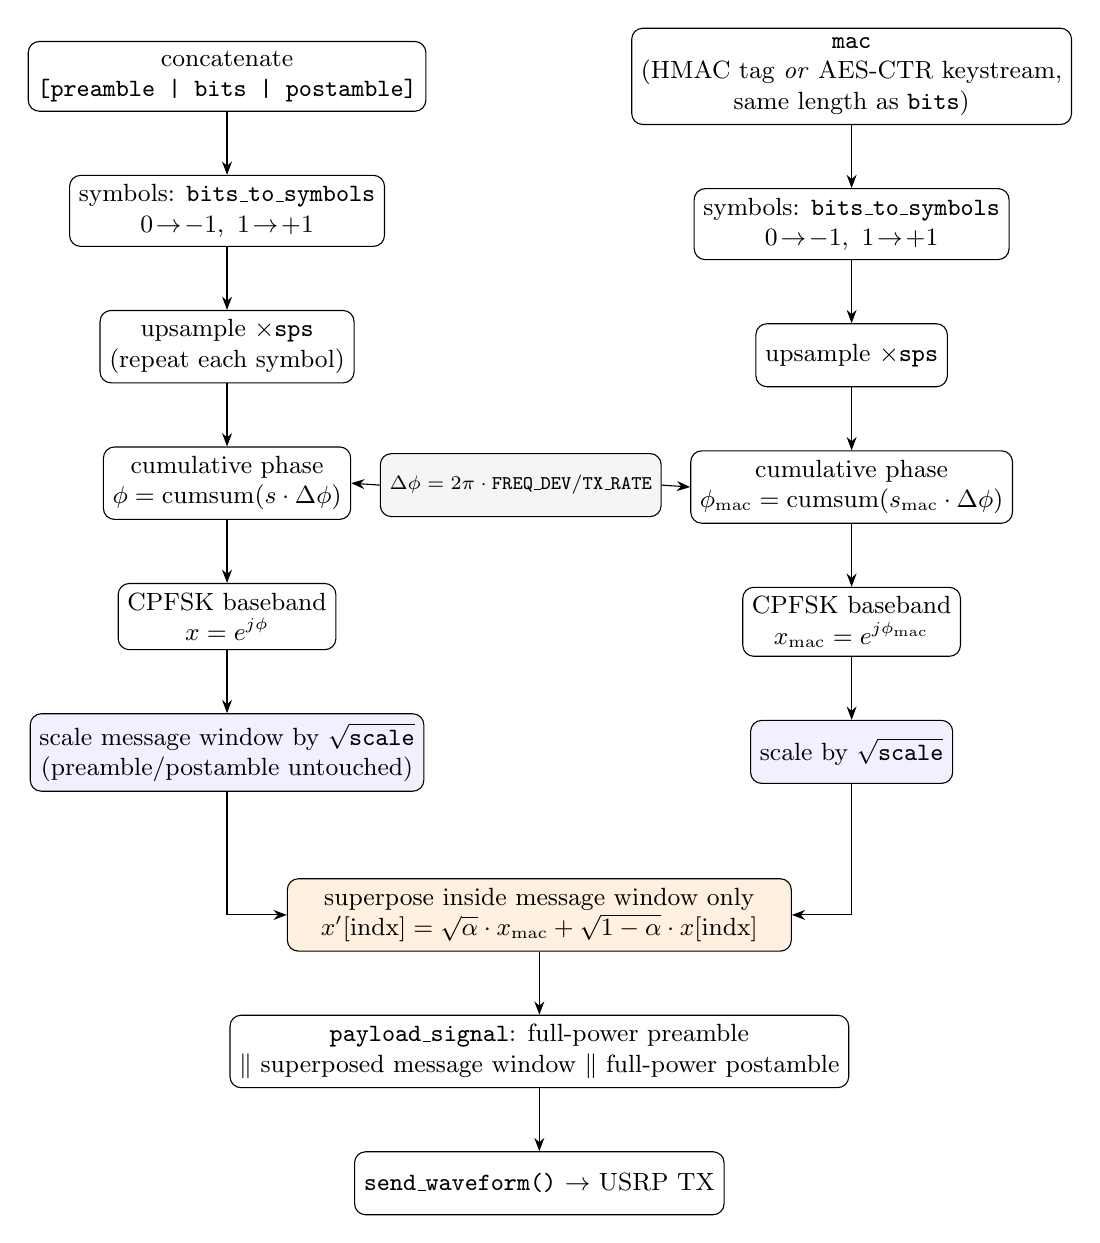
\begin{tikzpicture}[
    node distance=8mm and 10mm,
    box/.style={draw, rounded corners, minimum height=8mm, align=center, font=\small, fill=white},
    tiny/.style={font=\scriptsize},
    >=Stealth
]

% ---- Pipeline 1: full frame (message), continuous phase ----
\node[box] (concat) {concatenate\\\texttt{[preamble | bits | postamble]}};
\node[box, below=of concat] (sym1) {symbols: \texttt{bits\_to\_symbols}\\$0\!\to\!-1,\ 1\!\to\!+1$};
\node[box, below=of sym1] (up1) {upsample $\times$\texttt{sps}\\(repeat each symbol)};
\node[box, below=of up1] (cs1) {cumulative phase\\$\phi = \mathrm{cumsum}(s\cdot\Delta\phi)$};
\node[box, below=of cs1] (exp1) {CPFSK baseband\\$x = e^{j\phi}$};
\node[box, below=of exp1, fill=blue!6] (scale1) {scale message window by $\sqrt{\texttt{scale}}$\\(preamble/postamble untouched)};

% ---- Pipeline 2: mac / tag-or-keystream, independent phase ----
\node[box, right=26mm of concat] (mac) {\texttt{mac}\\(HMAC tag \emph{or} AES-CTR keystream,\\same length as \texttt{bits})};
\node[box, below=of mac] (sym2) {symbols: \texttt{bits\_to\_symbols}\\$0\!\to\!-1,\ 1\!\to\!+1$};
\node[box, below=of sym2] (up2) {upsample $\times$\texttt{sps}};
\node[box, below=of up2] (cs2) {cumulative phase\\$\phi_{\mathrm{mac}} = \mathrm{cumsum}(s_{\mathrm{mac}}\cdot\Delta\phi)$};
\node[box, below=of cs2] (exp2) {CPFSK baseband\\$x_{\mathrm{mac}} = e^{j\phi_{\mathrm{mac}}}$};
\node[box, below=of exp2, fill=blue!6] (scale2) {scale by $\sqrt{\texttt{scale}}$};

% shared constant -- placed in the horizontal gap between the two lanes,
% at the same height as the two "cumulative phase" boxes, so its arrows
% are plain horizontal segments that can't be confused with the vertical
% cs->exp arrows in either lane.
\node[box, tiny, fill=gray!8, minimum width=30mm] (dphi) at ($(cs1.east)!0.5!(cs2.west)$)
  {$\Delta\phi = 2\pi\cdot\texttt{FREQ\_DEV}/\texttt{TX\_RATE}$};

% ---- Combine ----
\node[box, below=16mm of $(scale1)!0.5!(scale2)$, fill=orange!12, minimum width=64mm] (combine)
  {superpose inside message window only\\
   $x'[\mathrm{indx}] = \sqrt{\alpha}\cdot x_{\mathrm{mac}} + \sqrt{1-\alpha}\cdot x[\mathrm{indx}]$};

\node[box, below=8mm of combine, minimum width=64mm] (out)
  {\texttt{payload\_signal}: full-power preamble\\
   $\|$ superposed message window $\|$ full-power postamble};

\node[box, below=8mm of out] (usrp) {\texttt{send\_waveform()} $\to$ USRP TX};

% arrows
\draw[->] (concat) -- (sym1);
\draw[->] (sym1) -- (up1);
\draw[->] (up1) -- (cs1);
\draw[->] (cs1) -- (exp1);
\draw[->] (exp1) -- (scale1);

\draw[->] (mac) -- (sym2);
\draw[->] (sym2) -- (up2);
\draw[->] (up2) -- (cs2);
\draw[->] (cs2) -- (exp2);
\draw[->] (exp2) -- (scale2);

\draw[->] (dphi.west) -- (cs1.east);
\draw[->] (dphi.east) -- (cs2.west);

\draw[->] (scale1) |- (combine);
\draw[->] (scale2) |- (combine);
\draw[->] (combine) -- (out);
\draw[->] (out) -- (usrp);

\end{tikzpicture}
\end{document}
